\documentclass{article}
\usepackage[margin=1in]{geometry}
\usepackage{problemset}
\showsolntrue

% Custom commands
\newcommand{\R}{\mathbb{R}}
\newcommand{\X}{\mathcal{X}}
\newcommand{\Y}{\mathcal{Y}}
\newcommand{\E}{\mathbb{E}}
\newcommand{\V}{\text{Var}}
\renewcommand{\P}{\mathbb{P}}
\newcommand{\N}{\mathcal{N}}

\begin{document}

\pstitle{%
    MATH 189%
}{
    Homework 2%
}[due Wednesday, January 22 at 8:00AM]

\begin{probset}

% --- Problem 1 ---
\begin{prob}[\textbf{Conceptual exercise 3}]
    Suppose we have a data set with five predictors, $X_1 = GPA$, $X_2 = IQ$, $X_3 = Level$ (1 for College and 0 for High School), $X_4 = Interaction$ between GPA and IQ, and $X_5 = Interaction$ between GPA and Level. The response is starting salary after graduation (in thousands of dollars). Suppose we use least squares to fit the model, and get $\hat{\beta}_0 = 50$, $\hat{\beta}_1 = 20$, $\hat{\beta}_2 = 0.07$, $\hat{\beta}_3 = 35$, $\hat{\beta}_4 = 0.01$, and $\hat{\beta}_5 = -10$.

    \begin{subprobset}
        \begin{subprob}
            Which answer is correct, and why?
            \begin{enumerate}[label=\roman*]
                \item For a fixed value of IQ and GPA, high school graduates earn more, on average, than college graduates.
                \item For a fixed value of IQ and GPA, college graduates earn more, on average, than high school graduates.
                \item For a fixed value of IQ and GPA, high school graduates earn more, on average, than college graduates provided that the GPA is high enough.
                \item For a fixed value of IQ and GPA, college graduates earn more, on average, than high school graduates provided that the GPA is high enough.
            \end{enumerate}

            \begin{soln}
                (iii), high school graduates earn more when
                \begin{align*}
                    50 + 20(GPA) + 0.07(IQ) + 0.01(GPA)(IQ) &> 85 + 10(GPA) + 0.07(IQ) + 0.01(GPA)(IQ) \\
                    20(GPA) &> 35 + 10(GPA) \\
                    10(GPA) &> 35 \\
                    GPA &> 3.5
                \end{align*}
                Thus, high school graduates earn more when the GPA is greater than 3.5.
            \end{soln}
        \end{subprob}

        \begin{subprob}
            Predict the salary of a college graduate with IQ of 110 and a GPA of 4.0.

            \begin{soln}
                The equation for the salary of a college graduate with IQ of 110 and a GPA of 4.0 is
                \begin{align*}
                    \hat{y} &= 50 + 20(GPA) + 0.07(IQ) + 35(Level) + 0.01(GPA)(IQ) - 10(GPA)(Level) \\
                    &= 50 + 20(4.0) + 0.07(110) + 35(1) + 0.01(4.0)(110) - 10(4.0)(1) \\
                    &= 50 + 80 + 7.7 + 35 + 4.4 - 40 \\
                    &= 137.1
                \end{align*}
                Thus, the salary of a college graduate with IQ of 110 and a GPA of 4.0 is 137,100 dollars.
            \end{soln}
        \end{subprob}

        \begin{subprob}
            True or false: Since the coefficient for the GPA/IQ interaction term is very small, there is very little evidence of an interaction effect. Justify your answer.

            \begin{soln}
                False. We need more information to determine if the interaction effect is significant, such as the p-value of the interaction term. The key thing is that we are missing the sample size. If it were large enough, we could reject the null hypothesis that the interaction effect is 0.
            \end{soln}
        \end{subprob}
    \end{subprobset}
\end{prob}

\newpage

% --- Problem 2 ---
\begin{prob}[\textbf{Conceptual exercise 5}]
    Consider the fitted values that result from performing linear regression without an intercept. In this setting, the ith fitted value takes the form
    \[\hat{y}_i = x_i \hat{\beta},\]
    where
    \[\hat{\beta} = \frac{\sum_{i=1}^n x_i y_i}{\sum_{i=1}^n x_i^2}.\]
    Show that we can write
    \[\hat{y}_i = \sum_{i'=1}^n a_{i'} y_{i'}.\]
    What is $a_{i'}$? \textit{Note: We interpret this result by saying that the fitted values from linear regression are linear combinations of the response values.}

    \begin{soln}
        Subbing in $\hat{\beta}$ into the equation for $\hat{y}_i$, we get
        \begin{align*}
            \hat{y}_i &= x_i \left(\frac{\sum_{i=1}^n x_i y_i}{\sum_{i=1}^n x_i^2}\right) \\
            &= \sum_{i'=1}^n \frac{x_i x_{i'}}{\sum_{i=1}^n x_i^2} y_{i'} \\
            &= \sum_{i'=1}^n a_{i'} y_{i'}
        \end{align*}
        Thus, $a_{i'} = \displaystyle\frac{x_i x_{i'}}{\sum_{i=1}^n x_i^2}$.
    \end{soln}
\end{prob}

% --- Problem 3 ---
\begin{prob}[\textbf{Conceptual exercise 6}]
    Argue that in the case of simple linear regression, the least squares line always passes through the point $(\bar{x}, \bar{y})$.

    \begin{soln}
        We can prove this by using the definition of the intercept term, $\hat{\beta}_0 = \bar{y} - \hat{\beta}_1 \bar{x}$. Plugging this as well as $(\bar{x}, \bar{y})$ into the equation for $\hat{y}_i$, we get
        \begin{align*}
            \bar{y} = \hat{\beta}_0 + \hat{\beta}_1 \bar{x} = \bar{y} - \hat{\beta}_1 \bar{x} + \hat{\beta}_1 \bar{x} = \bar{y}
        \end{align*}
        Thus, the point $(\bar{x}, \bar{y})$ is on the least squares line.
    \end{soln}
\end{prob}

\newpage

% --- Problem 4 ---
\begin{prob}[\textbf{Conceptual exercise 7}]
    In the case of simple linear regression of $Y$ onto $X$, the $R^2$ statistic is equal to the square of the correlation between $X$ and $Y$. Prove that this is the case. For simplicity, you may assume that $\bar{x} = \bar{y} = 0$.

    \begin{soln}
        Using the definition of correlation and the $R^2$ statistic, we have
        \begin{align*}
            R^2 &= 1 - \frac{\sum_{i=1}^n (y_i - \hat{y}_i)^2}{\sum_{i=1}^n (y_i - \bar{y})^2} && \text{by definition of $R^2$} \\
            &= 1 - \frac{\sum_{i=1}^n (y_i - \hat\beta_1 x_i)^2}{\sum_{i=1}^n (y_i - \bar{y})^2} && \hat\beta_0 = \bar{y} - \hat\beta_1 \bar{x} = 0 \\
            &= 1 - \frac{\sum_{i=1}^n y_i^2 - 2\hat\beta_1 \sum_{i=1}^n x_iy_i + \hat\beta_1^2 \sum_{i=1}^n x_i^2}{\sum_{i=1}^n y_i^2} && \text{expanding the square} \\
            &= 1 - \frac{\sum_{i=1}^n y_i^2 - \frac{\left[ \sum_{i=1}^n x_iy_i \right]^2}{\sum_{i=1}^n x_i^2}}{\sum_{i=1}^n y_i^2} && \hat\beta_1 = \frac{\sum_{i=1}^n x_iy_i}{\sum_{i=1}^n x_i^2} \\
            &= \frac{\left[ \sum_{i=1}^n x_iy_i \right]^2}{\sum_{i=1}^n x_i^2 \sum_{i=1}^n y_i^2} = r^2 && \text{by definition of correlation}
        \end{align*}
    \end{soln}
\end{prob}

% --- Problem 5 ---
\begin{prob}[\textbf{Applied exercise 13}]
    In this exercise you will create some simulated data and will fit simple linear regression models to it. Make sure to use the default random number generator with seed set to 1 prior to starting part (a) to ensure consistent results.

    \begin{subprobset}
        \begin{subprob}
            Using the \texttt{normal()} method of your random number generator, create a vector, $\texttt{x}$, containing 100 observations drawn from a $\N(0, 1)$ distribution. This represents a feature, $X$.

            \begin{soln}
                Check the code attached to the end.
            \end{soln}
        \end{subprob}

        \begin{subprob}
            Using the \texttt{normal()} method, create a vector, $\texttt{eps}$, containing 100 observations drawn from a $\N(0, 0.25)$ distribution - a normal distribution with mean zero and variance 0.25.

            \begin{soln}
                Check the code attached to the end.
            \end{soln}
        \end{subprob}

        \begin{subprob}
            Using $\texttt{x}$ and $\texttt{eps}$, generate a vector $\texttt{y}$ according to the model
            \[Y = -1 + 0.5X + \epsilon.\]
            What is the length of the vector $\texttt{y}$? What are the values of $\beta_0$ and $\beta_1$ in this linear model?

            \begin{soln}
                The length of the vector $\texttt{y}$ is 100 since \texttt{x} and \texttt{eps} have 100 elements. The values of $\beta_0$ and $\beta_1$ in this linear model are -1 and 0.5, respectively. We are given these in the definition of the model.
            \end{soln}
        \end{subprob}

        \newpage

        \begin{subprob}
            Create a scatterplot displaying the relationship between $\texttt{x}$ and $\texttt{y}$. Comment on what you observe.

            \begin{soln}
                \begin{center}
                    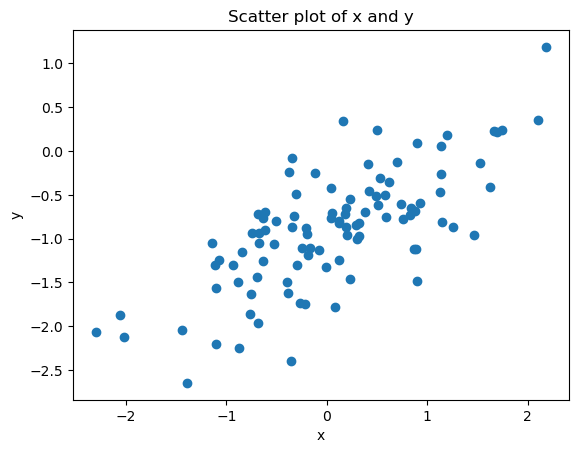
\includegraphics[width=0.5\textwidth]{Images/5d.png}
                \end{center}
                We can see that the relationship between $\texttt{x}$ and $\texttt{y}$ is linear and that most data is clustered together. However, there are a few outliers, most notably the one around $(2, 1)$. The data is also homoskedastic since the variance is constant across all values of $\texttt{x}$.
            \end{soln}
        \end{subprob}

        \begin{subprob}
            Fit a least squares linear model to predict $\texttt{y}$ using $\texttt{x}$. Comment on the model obtained. How do $\hat{\beta}_0$ and $\hat{\beta}_1$ compare to $\beta_0$ and $\beta_1$?

            \begin{soln}
                The model obtained is $\hat\beta_0 = -0.9265$ and $\hat\beta_1 = 0.5477$. These are very close to the true values of $\beta_0 = -1$ and $\beta_1 = 0.5$, respectively.
            \end{soln}
        \end{subprob}

        \begin{subprob}
            Display the least squares line on the scatterplot obtained in (d). Draw the population regression line on the plot, in a different color. Use the \texttt{legend()} method of the axes to create an appropriate legend.

            \begin{soln}
                \begin{center}
                    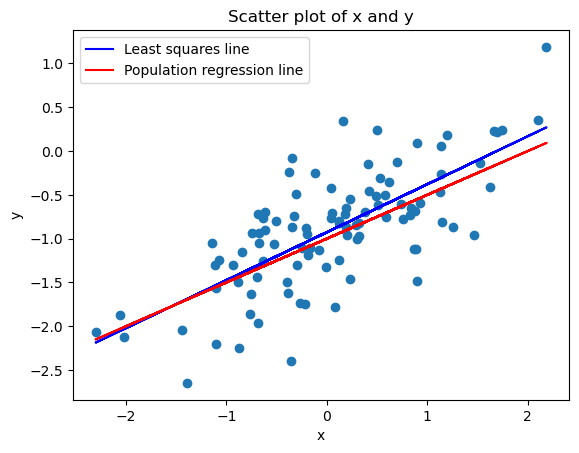
\includegraphics[width=0.5\textwidth]{Images/5f.png}
                \end{center}
                We can see that the least squares line is very close to the population regression line.
            \end{soln}
        \end{subprob}

        \newpage

        \begin{subprob}
            Now fit a polynomial regression model that predicts $\texttt{y}$ using $\texttt{x}$ and $\texttt{x}^2$. Is there evidence that the quadratic term improves the model fit? Explain your answer.

            \begin{soln}
                The model obtained is $\hat\beta_0 = -0.9325$, $\hat\beta_1 = 0.5468$, and $\hat\beta_2 = 0.0077$. The p-value for the quadratic term is 0.856, which is much more than 0.05. Therefore, there is no evidence that the quadratic term improves the model fit.
            \end{soln}
        \end{subprob}

        \begin{subprob}
            Repeat (a)-(f) after modifying the data generation process in such a way that there is less noise in the data. The model (1) should remain the same. You can do this by decreasing the variance of the normal distribution used to generate the error term $\epsilon$ in (b). Describe your results.

            \begin{soln}
                \begin{center}
                    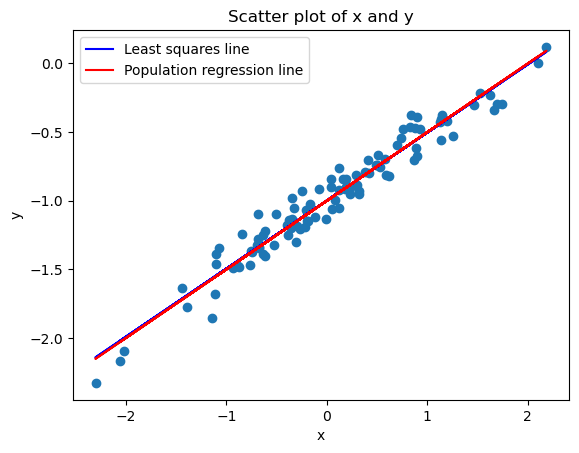
\includegraphics[width=0.7\textwidth]{Images/5h.png}
                \end{center}
                The values of $\beta_0$ and $\beta_1$ in this linear model are -0.9988 and 0.4959, respectively. These are even closer to the true values than the previous model since the noise is only 0.1 instead of 0.5. This can also be seen in the plot where the least squares line is even closer to the population regression line than the previous model.
            \end{soln}
        \end{subprob}

        \newpage

        \begin{subprob}
            Repeat (a)-(f) after modifying the data generation process in such a way that there is more noise in the data. The model (1) should remain the same. You can do this by increasing the variance of the normal distribution used to generate the error term $\epsilon$ in (b). Describe your results.

            \begin{soln}
                \begin{center}
                    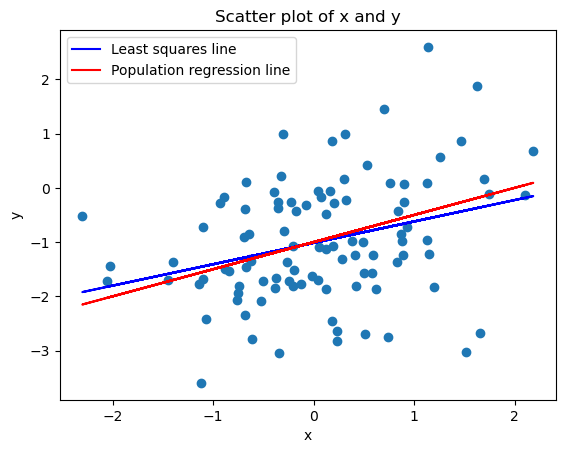
\includegraphics[width=0.7\textwidth]{Images/5i.png}
                \end{center}
                By increasing the noise (variance 1.0 instead of 0.25), the data becomes more spread out. The values of $\beta_0$ and $\beta_1$ in this linear model are -1.0140 and 0.3943, respectively. While the first value is close to the true value, the second value is not. This can also be seen in the plot where the least squares line is not as close to the population regression line as the previous model.
            \end{soln}
        \end{subprob}

        \begin{subprob}
            What are the confidence intervals for $\beta_0$ and $\beta_1$ based on the original data set, the noisier data set, and the less noisy data set? Comment on your results.

            \begin{soln}
                The 95\% confidence intervals based on the original data set are (-1.020, -0.833) for $\beta_0$ and (0.443, 0.653) for $\beta_1$. 
                
                The less noisy data intervals are (-1.019, -0.979) for $\beta_0$ and (0.473, 0.519) for $\beta_1$. 
                
                The noisier data intervals are (-1.227, -0.801) for $\beta_0$ and (0.154, 0.634) for $\beta_1$.

                As expected, the confidence intervals are narrower for the less noisy data set and wider for the noisier data set.
            \end{soln}
        \end{subprob}
    \end{subprobset}
\end{prob}

\newpage

% --- Problem 6 ---
\begin{prob}[\textbf{Applied exercise 15}]
    This problem involves the \texttt{Boston} data set, which we saw in the lab for this chapter. We will now try to predict per capita crime rate using the other variables in this data set. In other words, per capita crime rate is the response, and the other variables are the predictors.

    \begin{subprobset}
        \begin{subprob}
            For each predictor, fit a simple linear regression model to predict the response. Describe your results. In which of the models is there a statistically significant association between the predictor and the response? Create some plots to back up your assertions.

            \begin{soln}
                \begin{center}
                    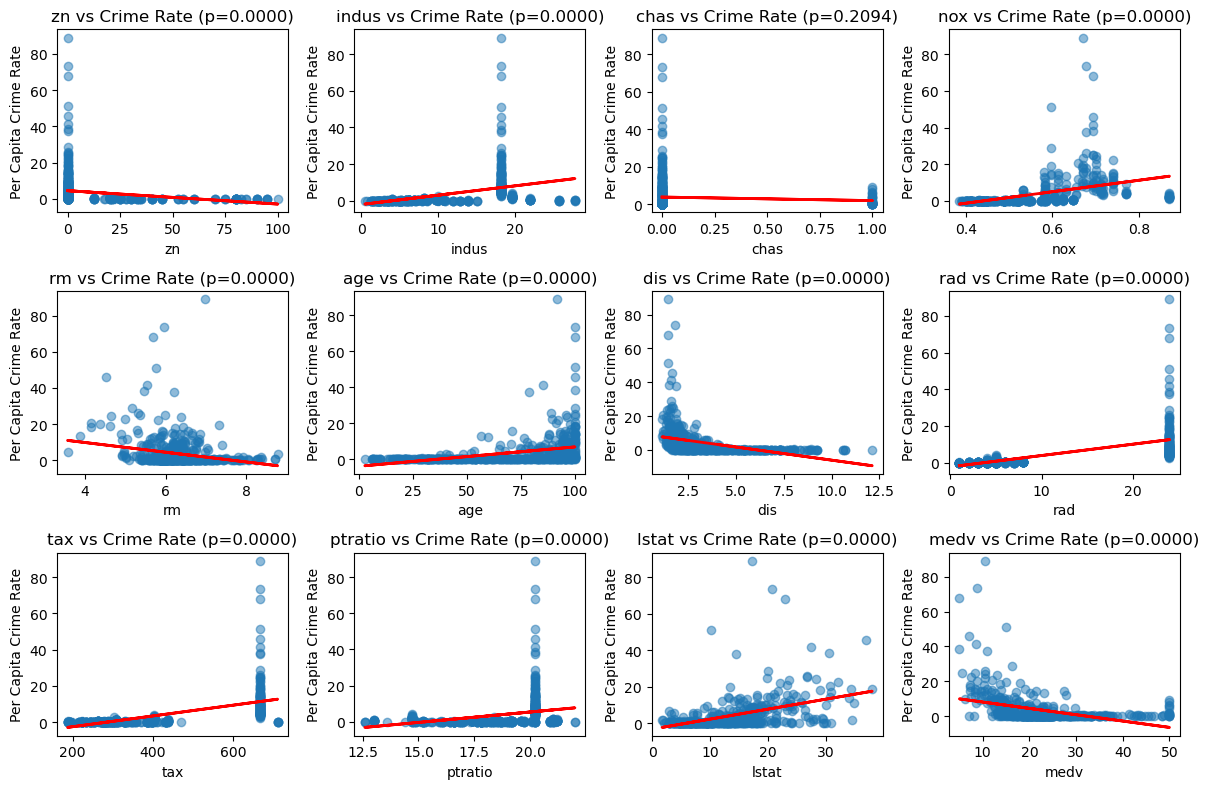
\includegraphics[width=0.8\textwidth]{Images/6a.png}
                \end{center}
                Running simple linear regression models for each predictor, we can see that every predictor except for \texttt{chas} is statistically significant at the 5\% level. This is interesting since \texttt{chas} is the only binary variable in this dataset.
            \end{soln}
        \end{subprob}

        \begin{subprob}
            Fit a multiple regression model to predict the response using all of the predictors. Describe your results. For which predictors can we reject the null hypothesis $H_0 : \beta_j = 0$?

            \begin{soln}
                Running multiple linear regression models for all predictors, we see almost the opposite results. Now only \texttt{zn}, \texttt{rad}, \texttt{dis}, and \texttt{medv} are statistically significant at the 5\% level. The $R^2$ is 0.449, which indicates that 44.9\% of the variance in crime rate is explained by the predictors.
            \end{soln}
        \end{subprob}

        \newpage

        \begin{subprob}
            How do your results from (a) compare to your results from (b)? Create a plot displaying the univariate regression coefficients from (a) on the x-axis, and the multiple regression coefficients from (b) on the y-axis. That is, each predictor is displayed as a single point in the plot. Its coefficient in a simple linear regression model is shown on the x-axis, and its coefficient estimate in the multiple linear regression model is shown on the y-axis.

            \begin{soln}
                \begin{center}
                    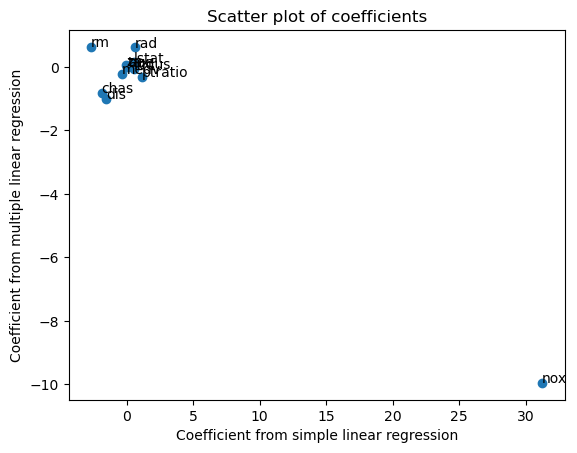
\includegraphics[width=0.8\textwidth]{Images/6c.png}
                \end{center}
                While almost all predictors were statistically significant in the simple linear regression model, only a few were statistically significant in the multiple linear regression model. Looking at the plot, we can see that most coefficients cluster around the origin, indicating that the predictors themselves are pretty weak. Some predictors like \texttt{rm} and \texttt{ptratio} even switch signs between the two models. The clear outlier is \texttt{nox}, which recieved opposite signs in the two models as well as extreme coefficients.
            \end{soln}
        \end{subprob}

        \newpage

        \begin{subprob}
            Is there evidence of non-linear association between any of the predictors and the response? To answer this question, for each predictor $X$, fit a model of the form
            \[Y = \beta_0 + \beta_1X + \beta_2X^2 + \beta_3X^3 + \epsilon.\]

            \begin{soln}
                \begin{center}
                    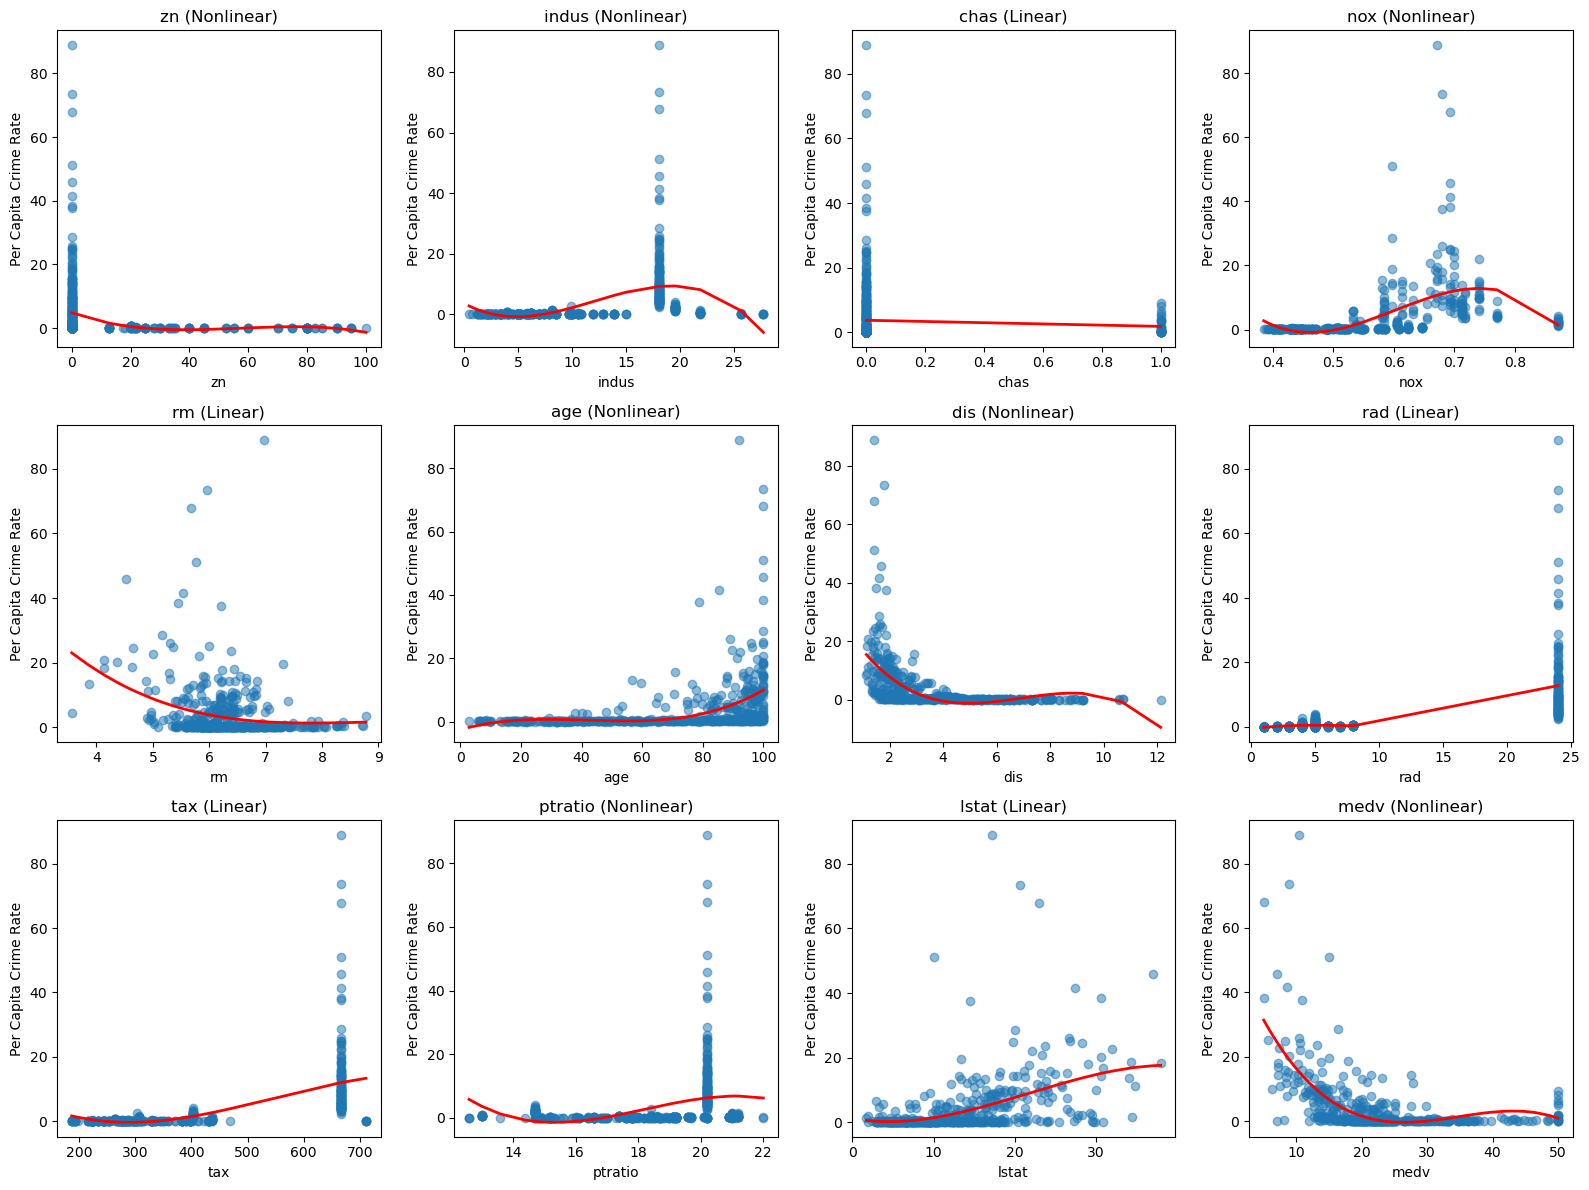
\includegraphics[width=0.8\textwidth]{Images/6d.png}
                \end{center}
                We can see that there is evidence of non-linear association between \texttt{zn}, \texttt{indus}, \texttt{nox}, \texttt{age}, \texttt{dis}, \texttt{ptratio}, and \texttt{medv}. The other predictors have p-values above 0.05 for both the quadratic and cubic terms, indicating that there is no evidence of non-linear association.
            \end{soln}
        \end{subprob}
    \end{subprobset}
\end{prob}
\end{probset}
\end{document}